\documentclass[aps,prl,twocolumn,superscriptaddress,nofootinbib]{revtex4-2}
\usepackage{amsmath,amssymb,amsfonts}
\usepackage{graphicx}
\usepackage{hyperref}
\usepackage{siunitx}

% Auto-generated by update_counts.py — 2026-10-14T09:43:30.211762
% Do not edit manually. Run: uv run python scripts/update_counts.py
\newcommand{\leantoolchain}{4.32.0}
\newcommand{\mathlibrev}{81a5d257}
\newcommand{\physlibrev}{c4843367}
\newcommand{\totaltheorems}{26353}
\newcommand{\substantivetheorems}{26327}
\newcommand{\placeholdertheorems}{26}
\newcommand{\kernelsubstantivetheorems}{26258}
\newcommand{\trackedvacuitydebt}{69}
\newcommand{\axiomcount}{0}
\newcommand{\sorrycount}{0}
\newcommand{\sorrypercent}{0.0}
\newcommand{\leanmodules}{2101}
\newcommand{\leandefinitions}{14045}
\newcommand{\pythonmodules}{138}
\newcommand{\testfiles}{214}
\newcommand{\totaltests}{7673}
\newcommand{\figurecount}{170}
\newcommand{\notebookcount}{91}
\newcommand{\papercount}{42}
\newcommand{\aristotleproved}{313}
\newcommand{\aristotleruns}{40}
% --- D11 bundle substrate summary (source-level, stated rule) ---
\newcommand{\dxiModules}{22}
\newcommand{\dxiLines}{6267}
\newcommand{\dxiTheorems}{403}
\newcommand{\dxiDefs}{82}
\newcommand{\dxiDepsTheorems}{409}
% --- Paper 18 / Phase 5t per-section counts (FermiHubbardDimer.lean) ---
\newcommand{\fhdTotal}{130}
\newcommand{\fhdWaveTwo}{13}
\newcommand{\fhdWaveThree}{6}
\newcommand{\fhdWaveFour}{19}
\newcommand{\fhdWaveFive}{20}
\newcommand{\fhdWaveSixABC}{35}
\newcommand{\fhdWaveSixExtra}{13}
\newcommand{\fhdWaveSeven}{17}
\newcommand{\fhdWaveEight}{7}
% --- Paper 26 / 27 per-module counts (BH entropy + four laws) ---
\newcommand{\bhEntropyTotal}{32}
\newcommand{\bhThermoTotal}{20}
% --- Phase 6 per-module + pytest counts (paper32 / paper34-38 / note_rt_ch_bounds) ---
\newcommand{\strongCpDeThms}{8}
\newcommand{\strongCpDeTests}{14}
\newcommand{\epThms}{24}
\newcommand{\epTests}{38}
\newcommand{\qecHolographyThms}{10}
\newcommand{\qecHolographyTests}{30}
\newcommand{\centerSymmThms}{18}
\newcommand{\centerSymmTests}{28}
\newcommand{\chiralSsbThms}{10}
\newcommand{\chiralSsbTests}{14}
\newcommand{\cflThms}{12}
\newcommand{\cflTests}{17}
\newcommand{\rtChThms}{7}
\newcommand{\rtChTests}{29}
\newcommand{\heatKernelThms}{20}
\newcommand{\heatKernelTests}{39}
\newcommand{\higherCurvatureThms}{13}
\newcommand{\higherCurvatureTests}{42}
\newcommand{\diffInvarianceThms}{13}
\newcommand{\diffInvarianceTests}{36}
\newcommand{\nonlinearEFEThms}{13}
\newcommand{\nonlinearEFETests}{40}
\newcommand{\microscopicCoefficientMatchThms}{12}
\newcommand{\microscopicCoefficientMatchTests}{42}
\newcommand{\einsteinCartanExtensionThms}{12}
\newcommand{\einsteinCartanExtensionTests}{41}
\newcommand{\bbnThms}{14}
\newcommand{\bbnTests}{16}
% --- Phase 6f/6g classical-GR per-module + wave totals (I1 §11–§13) ---
\newcommand{\curvatureThms}{14}
\newcommand{\einsteinTensorThms}{9}
\newcommand{\energyConditionsThms}{8}
\newcommand{\exactSolutionsThms}{16}
\newcommand{\admFormalismThms}{10}
\newcommand{\tetradFormalismThms}{5}
\newcommand{\phaseSixfWonesixTotal}{62}
\newcommand{\phaseSixfWsevenTotal}{13}
\newcommand{\riemannCoordinateThms}{8}
\newcommand{\riemannDifferentialBianchiThms}{8}
\newcommand{\bundleRiemannAuxThms}{6}
\newcommand{\bundleRiemannThms}{7}
\newcommand{\leviCivitaThms}{7}
\newcommand{\phaseSixfWeightTotal}{36}
\newcommand{\riccatiComparisonThms}{11}
\newcommand{\mazurSigmaModelRigidityThms}{12}
\newcommand{\hawkingPenroseCurveThms}{6}
\newcommand{\areaTheoremCurveThms}{10}
\newcommand{\phaseSixgWnineTotal}{39}
% --- D2 chirality-bundle per-module theorem counts (same convention as \totaltheorems) ---
\newcommand{\dtwoSmFermionDataThms}{19}
\newcommand{\dtwoZsixteenAnomalyThms}{23}
\newcommand{\dtwoVecGMonoidalThms}{11}
\newcommand{\dtwoToricCodeCenterThms}{25}
\newcommand{\dtwoCenterEquivalenceThms}{10}
\newcommand{\dtwoGoltermanShamirThms}{32}
\newcommand{\dtwoLatticeHamiltonianThms}{33}
\newcommand{\dtwoTpfEvasionThms}{14}
\newcommand{\dtwoPauliMatricesThms}{15}
\newcommand{\dtwoBdgHamiltonianThms}{8}
\newcommand{\dtwoChiralityWallMasterThms}{16}
\newcommand{\dtwoOnsagerAlgebraThms}{41}
\newcommand{\dtwoOnsagerContractionThms}{12}
\newcommand{\dtwoGtWeylDoubletThms}{15}
\newcommand{\dtwoFkGappedInterfaceThms}{12}
% --- paper10 per-module theorem counts (same convention as \totaltheorems) ---
\newcommand{\paperTenWangBridgeThms}{8}
\newcommand{\paperTenModularInvarianceThms}{11}
% --- Cross-platform Lean theorem reuse, 1+1D BEC -> 2+1D graphene (D1) ---
% Owner: scripts/count_theorem_reuse.py (population = the nine
% 1+1D BEC modules; REUSED = statement is platform-parametric).
\newcommand{\reuseTransferred}{107}
\newcommand{\reusePopulation}{120}
\newcommand{\reuseSpecific}{13}
\newcommand{\reusePercent}{89.17}
\newcommand{\reusePercentRounded}{89}
\newcommand{\reuseSpecificPercentRounded}{11}


%% ═══════════════════════════════════════════════════════════════════
%% Bundle: E1 (tier 4, target PRL | PRR)
%% Source manifest: papers/E1/source_manifest.md
%% Charter: docs/PAPER_STRATEGY.md §2.5 "Paper E1"
%%
%% STAGE-10 FULL REDRAFT — 2026-08-15. The prior draft is superseded in
%% full. Findings raised by this redraft:
%%   papers/AutomatedReviews/2026-08-15-e1-stage10-redraft/E1.md
%%
%% SPINE (derive before spend):
%%   §I    the opportunity, the obstacle, and what this Letter delivers
%%   §II   measured device parameters -> kappa, D, T_H            [derives]
%%   §III  the perturbative-dissipation criterion, evaluated       [derives]
%%   §IV   the stimulated-gain spectrum and its threshold          [spends]
%%   §V    noise floor and the falsifiable window                  [spends]
%%   §VI   what we need measured
%%   §VII  conclusion
%% ═══════════════════════════════════════════════════════════════════

%% GENERATED by scripts/render_bundle_counts.py — do not edit.
%% Per-bundle substrate counts, derived from this bundle's declared apex closure
%% (papers/<CODE>/bundle_metadata.json -> apex_theorems -> lean_deps.json).
%% Use these for any statement about THIS paper's verified content.
%% \substantivetheorems in docs/counts.tex is PROJECT-wide; using it for a
%% paper-scoped claim overstates by orders of magnitude (TODO-D9).
%% Closure walks stop at `private` declarations, so these are lower bounds.
\newcommand{\bundleTheorems}{7}
\newcommand{\bundleDecls}{15}
\newcommand{\bundleModules}{1}


\begin{document}

\title{Cavity Lifetime Gates Analog Hawking Detection in
Exciton-Polariton Microcavities}

\author{J.~Roehm}
\affiliation{Independent Researcher}

\date{\today}

\begin{abstract}
Cavity loss limits tests of analog Hawking radiation in
exciton-polariton fluids. At the Paris-LKB smooth horizon, the
standard relation gives
$T_H = % AUTOGENERATED by scripts/render_paper_tables.py — do not edit by hand.
% Regenerate via `uv run python scripts/render_paper_tables.py` after
% changing any source data or the paper's tables.py SCALARS spec.
% Description: E1 abstract and §5: Hawking temperature at the smooth horizon, in mK, from formulas.polariton_hawking_temperature.
85
\unskip\,\si{\milli\kelvin}$.
The as-built cavity fails our weak-dissipation criterion; a
fixed-horizon lifetime above about
$% AUTOGENERATED by scripts/render_paper_tables.py — do not edit by hand.
% Regenerate via `uv run python scripts/render_paper_tables.py` after
% changing any source data or the paper's tables.py SCALARS spec.
% Description: E1 §3 and §6 — THE ASK: the cavity lifetime at which Gamma_pol = 0.1*kappa at the smooth horizon, in ps. tau = 1/(0.1*kappa).
143
\unskip\,\si{\pico\second}$ is required.
For such a cavity and a saturated greybody factor, stimulated gain
reaches one half at
$\omega/\kappa_{\rm eff} = % AUTOGENERATED by scripts/render_paper_tables.py — do not edit by hand.
% Regenerate via `uv run python scripts/render_paper_tables.py` after
% changing any source data or the paper's tables.py SCALARS spec.
% Description: E1 §4: ln(3)/(2 pi) — the omega/kappa_eff at which the Gamma=1 adopted gain reaches 1/2. The dimensionless crossing is conditional; the dimensional frequency scales with kappa_eff and changes for nonunit greybody.
0.175
\unskip$,
where $\kappa_{\rm eff}$ is the effective surface gravity.
We give a working band and required calibrations.
\end{abstract}

\maketitle

%% ══════════════════════════════════════════════════════════════════
\section{Introduction}

Analog Hawking radiation has been observed in atomic Bose-Einstein
condensates at $T_H \approx \SI{0.35}{\nano\kelvin}$
\cite{Steinhauer2016,deNova2019}, so far below every systematic in
the apparatus that the signal must be recovered from
density-density correlations accumulated over thousands of
realizations. Exciton-polariton fluids remove that constraint
rather than fighting it: their sound speed exceeds a dilute atomic
gas's by some eight orders of magnitude, and their horizons are
written optically, so the velocity gradient setting the surface
gravity is both large and adjustable, and predicted temperatures
lie in the \SI{0.1}{\kelvin} to \SI{1}{\kelvin} range
\cite{Gerace2012,Nguyen2015}.

Falque \emph{et al.}~\cite{Falque2025} have now built the horizon.
Their microcavity polariton fluid crosses from sub- to supersonic
flow along an optically imprinted velocity profile, the horizon
steepness is tuned all-optically between two measured values, and
negative-energy Bogoliubov modes are resolved in the supersonic
region, which is the kinematic signature that a horizon has formed
and that pair emission across it is possible. What the platform does
not yet have is a prediction sharp enough to falsify, and a
statement of the device conditions under which that prediction is
entitled to be believed.

This Letter quantifies a necessary device condition for the
Schwinger-Keldysh effective-field-theory (SK-EFT) analog-Hawking
spectrum to describe the published Paris-LKB parameters. The
as-built cavity lies outside the weak-dissipation expansion. We
derive the lifetime threshold at fixed horizon steepness and give
conditional stimulated-gain targets for a longer-lived cavity.
Testing them also requires a calibrated transfer function and
noise budget.

%% ══════════════════════════════════════════════════════════════════
\section{Device parameters and the predicted Hawking temperature}

%% Data source: papers/E1/tables.py -> render_paper_tables.py, which reads
%%   src/core/constants.py :: POLARITON_PLATFORMS['Paris_standard'] and
%%   src/core/constants.py :: FALQUE_STEEP_HORIZON_KAPPA,
%% and derives D = xi*kappa/c_s and delta_disp = -pi D^2/6 rather than
%% quoting either. Every number in this section is generated.
%% Primary-source verification (2026-08-15, page-level read of
%% Lit-Search/Phase-5w/primary-sources/Falque2025.pdf):
%%   p.5 §IV.A  "the healing length ... is typically 3.4 um upstream and
%%               4.0 um downstream"; "the speed of sound c_s(x) ~ 0.40 um/ps"
%%   p.5 §IV.A  "horizon steepness kappa = 0.07 ps^-1 (red) and 0.08 (purple)"
%%   p.5 §IV.B  "We measure M_u = 0.7 and M_d = 4, with kappa = 0.11 ps^-1"
%%   p.4 §III   "effective polariton mass at the working point, m* = 7.0e-35 kg"
%%   p.9 App.B1 "We measure a polariton decay rate hbar*gamma ~ 80 ueV"

We take the fluid parameters from Falque \emph{et al.}~\cite{Falque2025}
directly rather than re-deriving them. Their \S IV.1 reports a sound
speed $c_s \approx % AUTOGENERATED by scripts/render_paper_tables.py — do not edit by hand.
% Regenerate via `uv run python scripts/render_paper_tables.py` after
% changing any source data or the paper's tables.py SCALARS spec.
% Description: E1 abstract + §2: sound speed of the Paris-LKB fluid, in um/ps (m/s * 1e6 um/m / 1e12 ps/s = m/s / 1e6).
0.40
\unskip\,\si{\micro\meter/\pico\second}$
and a healing length $\xi \approx % AUTOGENERATED by scripts/render_paper_tables.py — do not edit by hand.
% Regenerate via `uv run python scripts/render_paper_tables.py` after
% changing any source data or the paper's tables.py SCALARS spec.
% Description: E1 abstract + §2: upstream healing length, in um.
3.4
\unskip\,\si{\micro\meter}$
upstream (\SI{4.0}{\micro\meter} downstream), measured on a fluid whose
effective polariton mass is $m^* = \SI{7.0e-35}{\kilo\gram}$. Two
horizon steepnesses are reported: a smooth configuration at
$\kappa = % AUTOGENERATED by scripts/render_paper_tables.py — do not edit by hand.
% Regenerate via `uv run python scripts/render_paper_tables.py` after
% changing any source data or the paper's tables.py SCALARS spec.
% Description: E1 abstract, §2, §5 and the Fig. 2 caption: smooth-horizon surface gravity, in s^-1, in math-mode scientific form.
7\times 10^{10}
\unskip\,\mathrm{s}^{-1}$ and a steep one at
$\kappa = % AUTOGENERATED by scripts/render_paper_tables.py — do not edit by hand.
% Regenerate via `uv run python scripts/render_paper_tables.py` after
% changing any source data or the paper's tables.py SCALARS spec.
% Description: E1 abstract and §2: steep-horizon surface gravity, in s^-1, in math-mode scientific form.
1.1\times 10^{11}
\unskip\,\mathrm{s}^{-1}$.

That sound speed is not a reservoir-free Bogoliubov estimate
rescaled after the fact: the dark excitonic reservoir is already
inside it, carried as $g_r n_r \approx 1.84\,gn$ through the
dispersion from which $c_s$ is extracted. Reservoir-free estimates
for this class of device reach
$\sim \SI{1.0}{\micro\meter/\pico\second}$, so the reservoir costs a
factor of about two and a half, but that reduction is the primary
source's result rather than
ours~\cite{Estrecho2021,Stepanov2019,Claude2023}.

\begin{center}
% AUTOGENERATED by scripts/render_paper_tables.py — do not edit by hand.
% Regenerate via `uv run python scripts/render_paper_tables.py` after
% changing any source data or the paper's tables.py spec.
% Description: E1 §2: the two Paris-LKB horizon configurations reported by the primary source, with the dispersion ratio D = xi*kappa/c_s derived rather than quoted
\begin{tabular}{lcc}
\hline
Configuration & $\kappa$ ($\SI{}{\per\second}$) & $D = \xi\kappa/c_s$ \\
\hline
Smooth horizon (baseline) & $7\times 10^{10}$ & 0.59 \\
Steep horizon (reach) & $1.1\times 10^{11}$ & 0.94 \\
\hline
\end{tabular}

\end{center}

The dimensionless ratio $D = \xi\kappa/c_s$ compares the horizon's
gradient scale to the healing length and controls how far the
hydrodynamic description can be trusted. It is
$% AUTOGENERATED by scripts/render_paper_tables.py — do not edit by hand.
% Regenerate via `uv run python scripts/render_paper_tables.py` after
% changing any source data or the paper's tables.py SCALARS spec.
% Description: E1 abstract, §2 and the Fig. 2 caption: dispersion ratio D = xi*kappa/c_s at the smooth horizon.
0.59
\unskip$ at the smooth horizon and
$% AUTOGENERATED by scripts/render_paper_tables.py — do not edit by hand.
% Regenerate via `uv run python scripts/render_paper_tables.py` after
% changing any source data or the paper's tables.py SCALARS spec.
% Description: E1 abstract and §2: dispersion ratio at the steep horizon.
0.94
\unskip$ at the steep one. We take the leading
dispersive correction to be
\begin{equation}
\delta_{\rm disp} = -c_1 D^2 ,
\qquad c_1 \equiv \frac{\pi}{6},
\label{eq:delta_disp}
\end{equation}
giving $% AUTOGENERATED by scripts/render_paper_tables.py — do not edit by hand.
% Regenerate via `uv run python scripts/render_paper_tables.py` after
% changing any source data or the paper's tables.py SCALARS spec.
% Description: E1 §2: adopted phenomenological shift -c_1 D^2 at the smooth horizon (signed).
-0.19
\unskip$ and
$% AUTOGENERATED by scripts/render_paper_tables.py — do not edit by hand.
% Regenerate via `uv run python scripts/render_paper_tables.py` after
% changing any source data or the paper's tables.py SCALARS spec.
% Description: E1 §2: adopted phenomenological shift at the steep horizon (signed).
-0.46
\unskip$ respectively.

The $D^2$ scaling is the established one: Coutant and Weinfurtner obtain
the leading correction to the effective temperature as
$O(\xi^2\kappa^2/c_s^2)$ in the adiabatic regime. The \emph{coefficient}
is not. No derivation of a universal $c_1$ exists, and none is possible in
the form Eq.~\eqref{eq:delta_disp} suggests: for a locally linear
velocity profile the near-horizon calculation returns
$\beta_\omega = e^{-\pi\omega/\kappa}\alpha_\omega$ exactly, so the
temperature is $\kappa/2\pi$ with no $D^2$ term at all, and a correction
appears only through the profile's non-linear part~\cite{Coutant2014}.
Corley and Jacobson, correspondingly, report numerically fitted powers
$(T_H/k_0)^p$ whose exponent is itself profile-dependent, $p \simeq 3$ and
$2$ for smooth profiles and $p \simeq 1$ for kinked
ones~\cite{CorleyJacobson1996}. What that literature establishes is the
robustness of $T_H$, not a coefficient. The value $c_1 = \pi/6$ is
therefore fixed here as a declared normalization of an $O(1)$
profile-dependent quantity. This value is used throughout the
computational and formal definitions, so every $\delta_{\rm disp}$
quoted below and in the companion papers uses the same normalization.
A reader who prefers a different $O(1)$
normalization should rescale every dispersive number in this paper by
$c_1/(\pi/6)$; the quadratic $\kappa$-scaling and the
dispersive-versus-dissipative ordering are unaffected.

The Hawking temperature follows from the surface gravity alone,
\begin{equation}
k_B T_H = \frac{\hbar \kappa}{2\pi} ,
\label{eq:T_H}
\end{equation}
which at the smooth horizon gives
$T_H = % AUTOGENERATED by scripts/render_paper_tables.py — do not edit by hand.
% Regenerate via `uv run python scripts/render_paper_tables.py` after
% changing any source data or the paper's tables.py SCALARS spec.
% Description: E1 abstract and §5: Hawking temperature at the smooth horizon, in mK, from formulas.polariton_hawking_temperature.
85
\unskip\,\si{\milli\kelvin}$.

Two qualifications attach to that number, and both come from the
primary source rather than from the theory.

The first is a normalization. Falque \emph{et al.} quote a Hawking
temperature of \SI{3}{\kelvin} for their smoothest horizon, and
their Eq.~(9) writes the emitted flux as
$1/(e^{\omega/2\pi\kappa}-1)$. That exponent corresponds to
$k_B T = h\kappa$, which at the same
$\kappa = % AUTOGENERATED by scripts/render_paper_tables.py — do not edit by hand.
% Regenerate via `uv run python scripts/render_paper_tables.py` after
% changing any source data or the paper's tables.py SCALARS spec.
% Description: E1 abstract, §2, §5 and the Fig. 2 caption: smooth-horizon surface gravity, in s^-1, in math-mode scientific form.
7\times 10^{10}
\unskip\,\mathrm{s}^{-1}$ evaluates to
$% AUTOGENERATED by scripts/render_paper_tables.py — do not edit by hand.
% Regenerate via `uv run python scripts/render_paper_tables.py` after
% changing any source data or the paper's tables.py SCALARS spec.
% Description: E1 §2: the smooth-horizon temperature under the primary source's normalization k_B T = h kappa, in K. Falque et al. print "3 K" for this configuration.
3.4
\unskip\,\si{\kelvin}$ and reproduces the
flux values they report. It exceeds Eq.~\eqref{eq:T_H} by
$(2\pi)^2 \approx % AUTOGENERATED by scripts/render_paper_tables.py — do not edit by hand.
% Regenerate via `uv run python scripts/render_paper_tables.py` after
% changing any source data or the paper's tables.py SCALARS spec.
% Description: E1 §2: (2 pi)^2, the ratio between the primary source's normalization and the standard one.
39
\unskip$. We use
Eq.~\eqref{eq:T_H}, the convention of the analog-gravity literature
the same paper cites~\cite{Visser1998,Unruh1981,Barcelo2011}, and we
flag the factor here so that a reader holding \SI{3}{\kelvin} in
mind does not read
$% AUTOGENERATED by scripts/render_paper_tables.py — do not edit by hand.
% Regenerate via `uv run python scripts/render_paper_tables.py` after
% changing any source data or the paper's tables.py SCALARS spec.
% Description: E1 abstract and §5: Hawking temperature at the smooth horizon, in mK, from formulas.polariton_hawking_temperature.
85
\unskip\,\si{\milli\kelvin}$ as a
disagreement about $\kappa$. The two papers agree on every measured
quantity; they normalize $T_H$ differently.

The second is that Eq.~\eqref{eq:T_H} is only an observable where
the spectrum is thermal, and at the steep horizon it is not. Falque
\emph{et al.} state that the steep-horizon spectrum is dominated by
nonlinear frequency dispersion and is therefore not thermal, which
$D = % AUTOGENERATED by scripts/render_paper_tables.py — do not edit by hand.
% Regenerate via `uv run python scripts/render_paper_tables.py` after
% changing any source data or the paper's tables.py SCALARS spec.
% Description: E1 abstract and §2: dispersion ratio at the steep horizon.
0.94
\unskip$ anticipates: the dispersive correction
Eq.~\eqref{eq:delta_disp} is then near one half and the expansion
that produced it has stopped converging. We therefore quote a
Hawking temperature at the smooth horizon only, and treat the steep
configuration as what the source shows it to be, a demonstration
that $\kappa$ is tunable, not a hotter black hole.

%% ══════════════════════════════════════════════════════════════════
\section{The cavity lifetime the measurement requires}

%% Lean anchors, statements read 2026-08-15 (not docstrings):
%%   PolaritonTier1.lean:84   attenuation_ge_one
%%       1 <= attenuationFactor p,  attenuationFactor p = exp(Gamma*L/v_g)
%%   PolaritonTier1.lean:115  attenuation_mono_Gamma
%%       p1.L = p2.L -> p1.v_g = p2.v_g -> p1.Gamma <= p2.Gamma ->
%%       attenuationFactor p1 <= attenuationFactor p2
%%   PolaritonTier1.lean:98   attenuation_eq_one_at_zero_decay
%%       p.Gamma_pol = 0 -> attenuationFactor p = 1
%%   PolaritonTier1.lean:196  polariton_tier1_fails_tmds
%%       (1/10 : R) <= validityRatio pennTmdPolaritonParams
%%   All four kernel-only; axiom closure {propext, Classical.choice,
%%   Quot.sound}; no project-local axioms, no tracked Props.

Propagation at decay rate $\Gamma_{\rm pol} = 1/\tau_{\rm cav}$
reduces the emitted occupation by the factor
\begin{equation}
A = \exp\!\left(\frac{\Gamma_{\rm pol} L}{v_g}\right),
\label{eq:attenuation}
\end{equation}
with $L$ the propagation distance and $v_g$ the group velocity.
The attenuation model relates emitted and measured occupations by
\begin{equation}
N_{\rm meas} = N_{\rm emit}/A,
\qquad N_{\rm emit} = A N_{\rm meas}.
\end{equation}
Recovery multiplies by $A$. Lean~4 checks three properties of this
defined factor for all admissible parameters:
$A \geq 1$ always, so the recovery never deflates an inferred
occupation (\texttt{attenuation\_ge\_one}); $A$ is monotone in
$\Gamma_{\rm pol}$ at fixed geometry
(\texttt{attenuation\_mono\_Gamma}); and $\Gamma_{\rm pol} = 0$ implies $A = 1$, the closed-system limit
(\texttt{attenuation\_eq\_one\_at\_zero\_decay}).
At zero propagation distance, $A = 1$ even with positive decay.

The SK-EFT dissipation expansion requires small
$\Gamma_{\rm pol}/\kappa$. We impose
\begin{equation}
\Gamma_{\rm pol} < % AUTOGENERATED by scripts/render_paper_tables.py — do not edit by hand.
% Regenerate via `uv run python scripts/render_paper_tables.py` after
% changing any source data or the paper's tables.py SCALARS spec.
% Description: E1 §3: the weak-dissipation criterion Gamma_pol < r*kappa; r as declared, matching the constants.py tier1_valid cut.
0.1
\unskip\,\kappa
\label{eq:weak_dissipation}
\end{equation}
as a declared validity convention, not a derived boundary.

Falque \emph{et al.} measure a polariton decay rate
$\hbar\gamma \approx \SI{80}{\micro\electronvolt}$, or
$\tau_{\rm cav} \approx % AUTOGENERATED by scripts/render_paper_tables.py — do not edit by hand.
% Regenerate via `uv run python scripts/render_paper_tables.py` after
% changing any source data or the paper's tables.py SCALARS spec.
% Description: E1 §3: as-built Paris-LKB cavity lifetime, in ps (Falque 2025 actual; hbar*gamma ~ 80 ueV, Appendix B.1).
8
\unskip\,\si{\pico\second}$.
Against $\kappa = % AUTOGENERATED by scripts/render_paper_tables.py — do not edit by hand.
% Regenerate via `uv run python scripts/render_paper_tables.py` after
% changing any source data or the paper's tables.py SCALARS spec.
% Description: E1 abstract, §2, §5 and the Fig. 2 caption: smooth-horizon surface gravity, in s^-1, in math-mode scientific form.
7\times 10^{10}
\unskip\,\mathrm{s}^{-1}$ this gives
\begin{equation}
\frac{\Gamma_{\rm pol}}{\kappa} = % AUTOGENERATED by scripts/render_paper_tables.py — do not edit by hand.
% Regenerate via `uv run python scripts/render_paper_tables.py` after
% changing any source data or the paper's tables.py SCALARS spec.
% Description: E1 §3 and the Fig. 2 caption: Gamma_pol/kappa at the as-built cavity and the smooth horizon. The paper headline.
1.79
\unskip ,
\label{eq:ratio_asbuilt}
\end{equation}
about eighteen times the cut. Over one healing length, the exponent
in Eq.~\eqref{eq:attenuation} is $(\Gamma_{\rm pol}/\kappa)D\,c_s/v_g$.
Taking $v_g = c_s$ gives the recovery factor
$% AUTOGENERATED by scripts/render_paper_tables.py — do not edit by hand.
% Regenerate via `uv run python scripts/render_paper_tables.py` after
% changing any source data or the paper's tables.py SCALARS spec.
% Description: E1 §3: exp(Gamma_pol xi / c_s) = exp(ratio*D), the occupation-recovery factor per healing length of propagation, at the as-built cavity, assuming v_g = c_s.
2.9
\unskip$. The per-healing-length
estimates here use this velocity identification.

At fixed horizon, a
\SI{100}{\pico\second} cavity gives
$\Gamma_{\rm pol}/\kappa = % AUTOGENERATED by scripts/render_paper_tables.py — do not edit by hand.
% Regenerate via `uv run python scripts/render_paper_tables.py` after
% changing any source data or the paper's tables.py SCALARS spec.
% Description: E1 §3: Gamma_pol/kappa for the PROJECTED 100 ps cavity.
0.14
\unskip$ and a
\SI{300}{\pico\second} cavity gives
$% AUTOGENERATED by scripts/render_paper_tables.py — do not edit by hand.
% Regenerate via `uv run python scripts/render_paper_tables.py` after
% changing any source data or the paper's tables.py SCALARS spec.
% Description: E1 §3: Gamma_pol/kappa for the PROJECTED 300 ps cavity.
0.048
\unskip$. Eq.~\eqref{eq:weak_dissipation}
is met from
\begin{equation}
\boxed{\;\tau_{\rm cav} \gtrsim
  % AUTOGENERATED by scripts/render_paper_tables.py — do not edit by hand.
% Regenerate via `uv run python scripts/render_paper_tables.py` after
% changing any source data or the paper's tables.py SCALARS spec.
% Description: E1 §3 and §6 — THE ASK: the cavity lifetime at which Gamma_pol = 0.1*kappa at the smooth horizon, in ps. tau = 1/(0.1*kappa).
143
\unskip\,\si{\pico\second}\;}
\label{eq:tau_required}
\end{equation}
onward, with per-healing-length recovery factor
$% AUTOGENERATED by scripts/render_paper_tables.py — do not edit by hand.
% Regenerate via `uv run python scripts/render_paper_tables.py` after
% changing any source data or the paper's tables.py SCALARS spec.
% Description: E1 §3: the same recovery factor per healing length at the weak-dissipation boundary Gamma_pol = 0.1 kappa, assuming v_g = c_s.
1.06
\unskip$. Availability of such a
GaAs cavity remains a fabrication question; the horizon is unchanged.
%% TODO: the claim that GaAs microcavities with tau_cav >= 143 ps are
%% demonstrated is NOT made here, because it is not verified. The
%% repo's PARAMETER_PROVENANCE cites Ballarini 2017 for long-lifetime
%% cavities, but only in support of the 100 ps projection, which is
%% BELOW this threshold, and that source is not held in full text.
%% Acquire it (and the higher-Q GaAs literature) before any future
%% draft asserts availability. Filed nowhere else deliberately: this
%% is a source-acquisition task, not a defect in the present text.

Figure~\ref{fig:regime} locates the GaAs devices. Outside that family,
the UPenn MoSe$_2$ nanocavity of Wang \emph{et
al.}~\cite{WangKimBZHe2026PennTMDPolariton}, whose lower-polariton
linewidth $\gamma_{\rm LP} = \SI{1.8}{\milli\electronvolt}$ implies
$\Gamma_{\rm LP} \approx \SI{2.7e12}{\per\second}$, sits at
$\Gamma_{\rm LP}/\kappa = % AUTOGENERATED by scripts/render_paper_tables.py — do not edit by hand.
% Regenerate via `uv run python scripts/render_paper_tables.py` after
% changing any source data or the paper's tables.py SCALARS spec.
% Description: E1 §3: Penn TMD nanocavity Gamma_LP over the MOST GENEROUS polariton-family kappa (Falque steep), matching the Lean theorem polariton_tier1_fails_tmds.
24.9
\unskip$ even when
paired with the most generous surface gravity the polariton family
has demonstrated, so no SK-EFT statement in this Letter extends to
ultrafast TMD nanocavities. That the ratio there is at least
$% AUTOGENERATED by scripts/render_paper_tables.py — do not edit by hand.
% Regenerate via `uv run python scripts/render_paper_tables.py` after
% changing any source data or the paper's tables.py SCALARS spec.
% Description: E1 §3: the weak-dissipation criterion Gamma_pol < r*kappa; r as declared, matching the constants.py tier1_valid cut.
0.1
\unskip$ is itself kernel-checked
(\texttt{polariton\_tier1\_fails\_tmds}); the value
$% AUTOGENERATED by scripts/render_paper_tables.py — do not edit by hand.
% Regenerate via `uv run python scripts/render_paper_tables.py` after
% changing any source data or the paper's tables.py SCALARS spec.
% Description: E1 §3: Penn TMD nanocavity Gamma_LP over the MOST GENEROUS polariton-family kappa (Falque steep), matching the Lean theorem polariton_tier1_fails_tmds.
24.9
\unskip$ is arithmetic on the same
encoded parameters.

\begin{figure}[t]
\centering
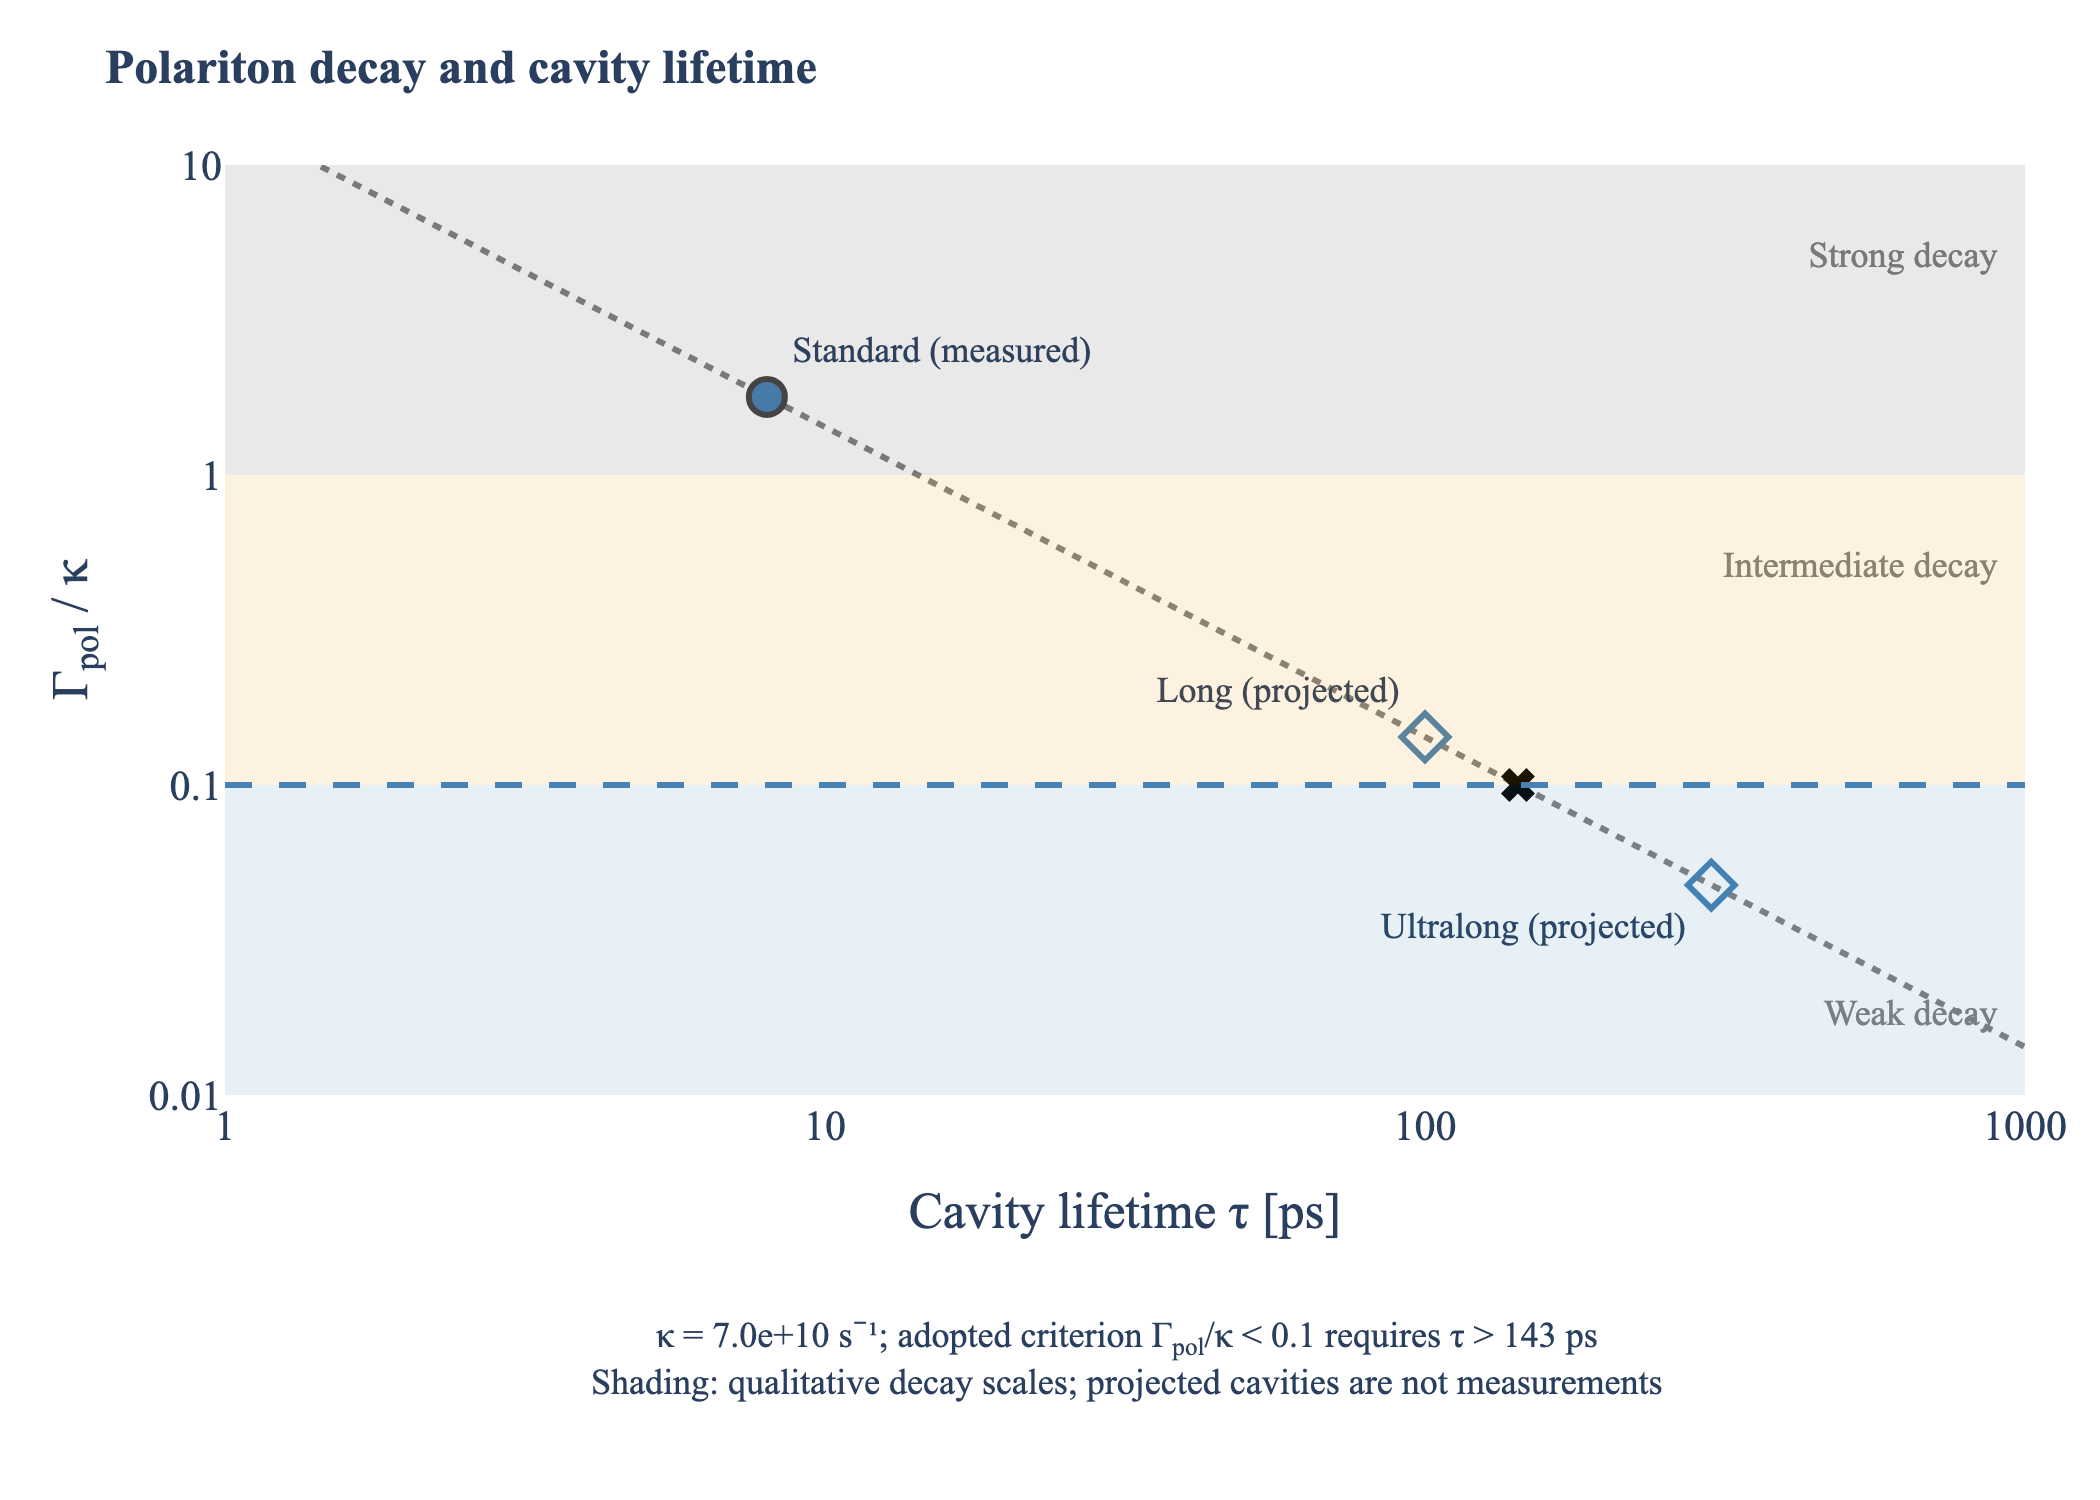
\includegraphics[width=\columnwidth]{figures/fig_polariton_regime_map.png}
\caption[The weak-dissipation criterion against cavity lifetime]{Normalized
polariton decay $\Gamma_{\rm pol}/\kappa$ against cavity lifetime
$\tau_{\rm cav}$, at the smooth-horizon
$\kappa = % AUTOGENERATED by scripts/render_paper_tables.py — do not edit by hand.
% Regenerate via `uv run python scripts/render_paper_tables.py` after
% changing any source data or the paper's tables.py SCALARS spec.
% Description: E1 abstract, §2, §5 and the Fig. 2 caption: smooth-horizon surface gravity, in s^-1, in math-mode scientific form.
7\times 10^{10}
\unskip\,\mathrm{s}^{-1}$ of
Falque \emph{et al.}~\cite{Falque2025}. The as-built
% AUTOGENERATED by scripts/render_paper_tables.py — do not edit by hand.
% Regenerate via `uv run python scripts/render_paper_tables.py` after
% changing any source data or the paper's tables.py SCALARS spec.
% Description: E1 §3: as-built Paris-LKB cavity lifetime, in ps (Falque 2025 actual; hbar*gamma ~ 80 ueV, Appendix B.1).
8
\unskip\,\si{\pico\second} device
(``standard'') sits at $% AUTOGENERATED by scripts/render_paper_tables.py — do not edit by hand.
% Regenerate via `uv run python scripts/render_paper_tables.py` after
% changing any source data or the paper's tables.py SCALARS spec.
% Description: E1 §3 and the Fig. 2 caption: Gamma_pol/kappa at the as-built cavity and the smooth horizon. The paper headline.
1.79
\unskip$, above unity,
where the weak-dissipation expansion of
Eq.~\eqref{eq:weak_dissipation} does not apply. The dotted trajectory
$\Gamma_{\rm pol}/\kappa = 1/(\tau_{\rm cav}\kappa)$ crosses the criterion
at Eq.~\eqref{eq:tau_required}. The
\SI{100}{\pico\second} (``long'') and \SI{300}{\pico\second}
(``ultralong'') points are projected cavity generations, not
measured devices. Shaded bands indicate qualitative decay scales.}
\label{fig:regime}
\end{figure}

The measured horizon fixes $\kappa$ independently of the cavity.
The leading-order temperature and gain expressions,
Eqs.~\eqref{eq:T_H} and~\eqref{eq:gain}, are predictions only when
the dissipation expansion applies. The gain magnitudes, occupation
recovery and window uncertainties in \S IV and \S V therefore assume
Eq.~\eqref{eq:tau_required}. They are targets for an improved cavity,
not predictions for the as-built device.

%% ══════════════════════════════════════════════════════════════════
\section{The stimulated-Hawking gain spectrum}

%% Numbers consumed from src/core/formulas.py :: stimulated_hawking_gain
%% and :: stimulated_hawking_snr via papers/E1/tables.py. The argument is
%% omega/kappa_eff, which is what the exponent contains.

Waiting for spontaneous emission is what makes the atomic-BEC
measurements slow, and driving the horizon removes that cost. A
coherent probe injected at frequency $\omega$ scatters anomalously
at the horizon, and the amplitude returned in the partner channel is
set by the same Bogoliubov mixing that produces the spontaneous
pairs, so a classical mean-field measurement reads out a
quantum-gravitational analog coefficient~\cite{Grisins2016}. The
gain is
\begin{equation}
G(\omega) = \frac{\Gamma(\omega)}{e^{2\pi\omega/\kappa_{\rm eff}} - 1},
\label{eq:gain}
\end{equation}
with $\Gamma(\omega)$ the greybody transmission factor and
$\kappa_{\rm eff} = \kappa\,(1 + \delta_{\rm disp})$ the surface
gravity carrying the dispersive correction of
Eq.~\eqref{eq:delta_disp}. At the smooth horizon
$\kappa_{\rm eff}/\kappa = % AUTOGENERATED by scripts/render_paper_tables.py — do not edit by hand.
% Regenerate via `uv run python scripts/render_paper_tables.py` after
% changing any source data or the paper's tables.py SCALARS spec.
% Description: E1 §4: adopted kappa_eff/kappa = 1 + delta_disp at the smooth horizon.
0.81
\unskip$.

Every number below assumes the greybody-saturation limit
$\Gamma(\omega) \equiv 1$. This is an adopted model for the
numerical illustration, not a measured transmission profile.
The hydrodynamic approximation alone does not establish its
accuracy over the chosen band. Independent calibration of
$\Gamma(\omega)$ and the detection transfer function is required
to test the predicted gain.

Under it the gain falls monotonically from a low-frequency
divergence: $G = % AUTOGENERATED by scripts/render_paper_tables.py — do not edit by hand.
% Regenerate via `uv run python scripts/render_paper_tables.py` after
% changing any source data or the paper's tables.py SCALARS spec.
% Description: E1 §4 and the Fig. 1 caption: G at omega = 0.1 kappa_eff, greybody-saturated.
1.14
\unskip$ at
$\omega = 0.1\,\kappa_{\rm eff}$,
$% AUTOGENERATED by scripts/render_paper_tables.py — do not edit by hand.
% Regenerate via `uv run python scripts/render_paper_tables.py` after
% changing any source data or the paper's tables.py SCALARS spec.
% Description: E1 §4: G at omega = 0.3 kappa_eff, greybody-saturated.
0.18
\unskip$ at $0.3\,\kappa_{\rm eff}$, and
$% AUTOGENERATED by scripts/render_paper_tables.py — do not edit by hand.
% Regenerate via `uv run python scripts/render_paper_tables.py` after
% changing any source data or the paper's tables.py SCALARS spec.
% Description: E1 §4: G at omega = kappa_eff, greybody-saturated. Two significant figures, matching its neighbours (the prior draft rounded this one to 0.002 and its neighbours to two).
0.0019
\unskip$ at $\kappa_{\rm eff}$. Setting
$G = 1/2$ inverts Eq.~\eqref{eq:gain} exactly, within this assumed limit:
\begin{equation}
\frac{\omega_{1/2}}{\kappa_{\rm eff}} = \frac{\ln 3}{2\pi}
  = % AUTOGENERATED by scripts/render_paper_tables.py — do not edit by hand.
% Regenerate via `uv run python scripts/render_paper_tables.py` after
% changing any source data or the paper's tables.py SCALARS spec.
% Description: E1 §4: ln(3)/(2 pi) — the omega/kappa_eff at which the Gamma=1 adopted gain reaches 1/2. The dimensionless crossing is conditional; the dimensional frequency scales with kappa_eff and changes for nonunit greybody.
0.175
\unskip .
\label{eq:threshold}
\end{equation}
The dimensionless ratio in Eq.~\eqref{eq:threshold} is independent
of $\kappa$ in the saturated-greybody model. The dimensional
frequency still scales with $\kappa_{\rm eff}$. Expressed relative
to the measured surface gravity, the adopted dispersive correction
gives $\omega_{1/2}/\kappa =
% AUTOGENERATED by scripts/render_paper_tables.py — do not edit by hand.
% Regenerate via `uv run python scripts/render_paper_tables.py` after
% changing any source data or the paper's tables.py SCALARS spec.
% Description: E1 §4: the same crossing expressed in absolute kappa units, ln(3)/(2 pi) * (1 + delta_disp) at the smooth horizon.
0.142
\unskip$ at the smooth
horizon. A nonunit greybody factor shifts the crossing: even a
constant $\Gamma$ gives
$\omega_{1/2}/\kappa_{\rm eff}=\ln(1+2\Gamma)/(2\pi)$.
Inferring a dispersive correction from this crossing therefore
requires independent calibration of transmission and detected gain.

\begin{figure}[t]
\centering
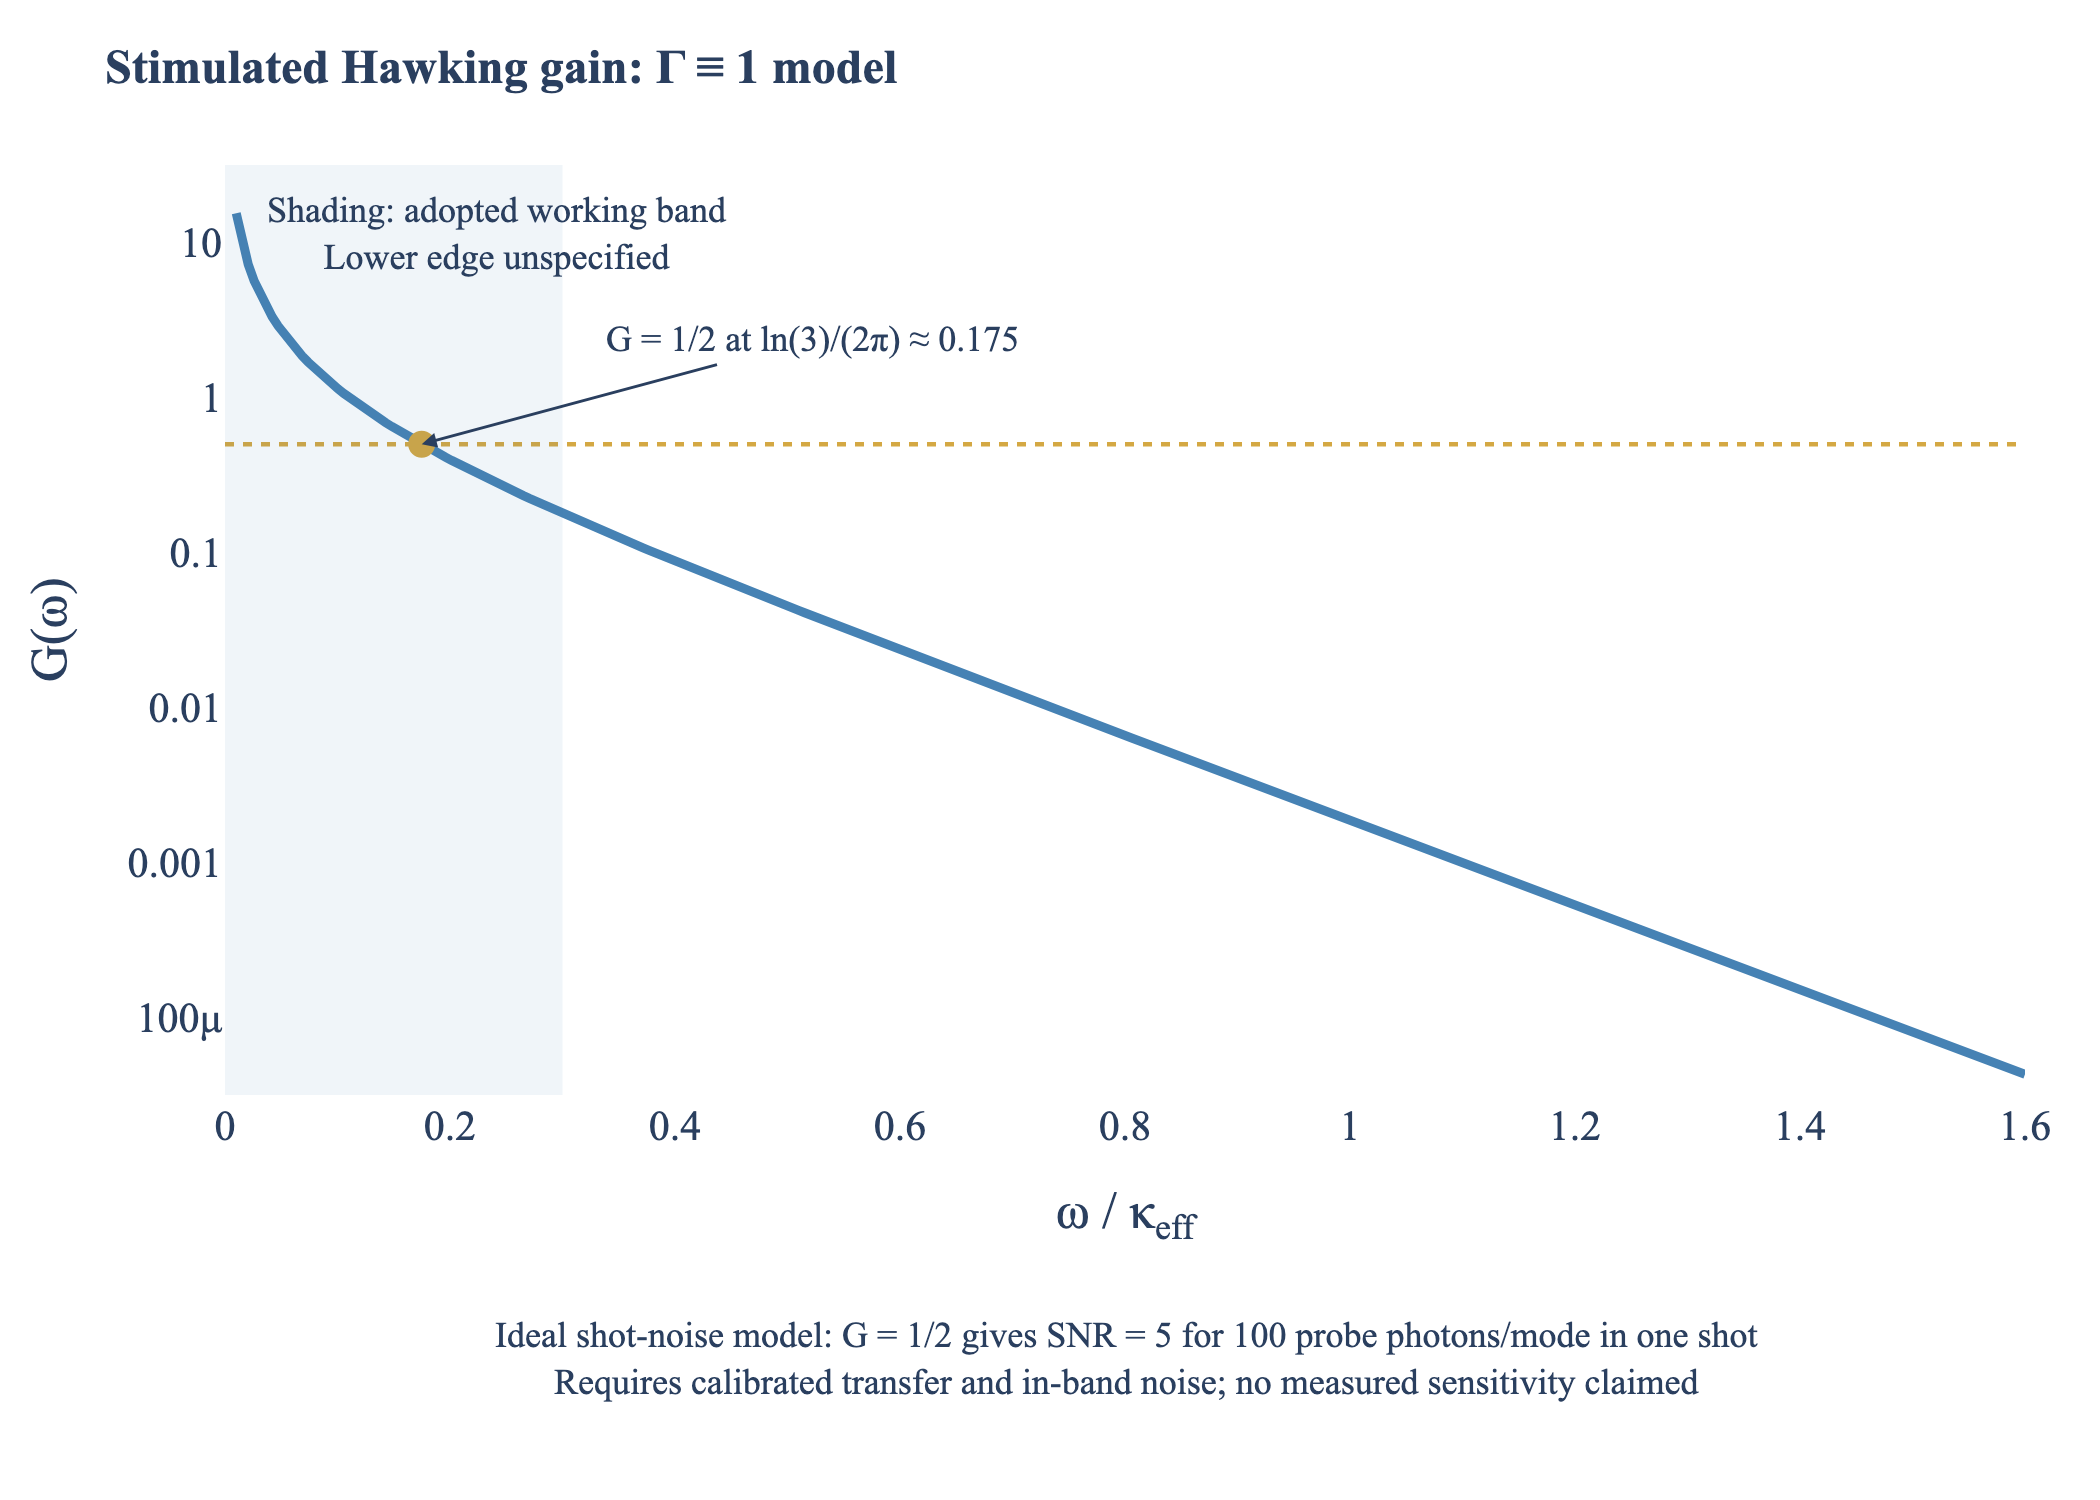
\includegraphics[width=\columnwidth]{figures/fig_stimulated_hawking_spectrum.png}
\caption[Stimulated-Hawking gain against normalized frequency]{Stimulated-Hawking
gain $G(\omega)$ against normalized frequency, at the smooth-horizon
$\kappa = % AUTOGENERATED by scripts/render_paper_tables.py — do not edit by hand.
% Regenerate via `uv run python scripts/render_paper_tables.py` after
% changing any source data or the paper's tables.py SCALARS spec.
% Description: E1 abstract, §2, §5 and the Fig. 2 caption: smooth-horizon surface gravity, in s^-1, in math-mode scientific form.
7\times 10^{10}
\unskip\,\mathrm{s}^{-1}$ and
$D = % AUTOGENERATED by scripts/render_paper_tables.py — do not edit by hand.
% Regenerate via `uv run python scripts/render_paper_tables.py` after
% changing any source data or the paper's tables.py SCALARS spec.
% Description: E1 abstract, §2 and the Fig. 2 caption: dispersion ratio D = xi*kappa/c_s at the smooth horizon.
0.59
\unskip$ of Falque \emph{et al.}~\cite{Falque2025},
in the greybody-saturation limit $\Gamma \equiv 1$. The abscissa is
$\omega/\kappa_{\rm eff}$, so the dashed $G=1/2$ crossing lies at
$\ln(3)/(2\pi)=% AUTOGENERATED by scripts/render_paper_tables.py — do not edit by hand.
% Regenerate via `uv run python scripts/render_paper_tables.py` after
% changing any source data or the paper's tables.py SCALARS spec.
% Description: E1 §4: ln(3)/(2 pi) — the omega/kappa_eff at which the Gamma=1 adopted gain reaches 1/2. The dimensionless crossing is conditional; the dimensional frequency scales with kappa_eff and changes for nonunit greybody.
0.175
\unskip$.
The ideal shot-noise model assigns $5\sigma$ to this gain with
100 probe photons per mode; this is conditional on the calibrated
readout, not demonstrated detector performance. Shading denotes
the adopted working band of Eq.~\eqref{eq:window}, not a derived
validity bound. Its unresolved lower edge is not shown.}
\label{fig:gain}
\end{figure}

For an ideal shot-noise-limited readout we adopt
$\mathrm{SNR}=\sqrt{N_{\rm shots}N_{\rm probe}}\;G(\omega)$.
This model assigns a single-shot $5\sigma$ significance to
$G=1/2$ with 100 probe photons per mode, and
$\mathrm{SNR}=% AUTOGENERATED by scripts/render_paper_tables.py — do not edit by hand.
% Regenerate via `uv run python scripts/render_paper_tables.py` after
% changing any source data or the paper's tables.py SCALARS spec.
% Description: E1 §4: ideal shot-noise SNR at omega = 0.1 kappa_eff with 100 probe photons per mode; not calibrated detector significance.
11
\unskip$ at
$\omega=0.1\,\kappa_{\rm eff}$. These are conditional readout
estimates. Applying them to detected counts requires the collection
and detection efficiencies, transfer function and measured
background to be included in the noise budget.

%% ══════════════════════════════════════════════════════════════════
\section{Noise budget and the working frequency band}

The mean-field energy expressed in temperature units is
\begin{equation}
T_{\rm mf}=\frac{m^*c_s^2}{k_B}
=% AUTOGENERATED by scripts/render_paper_tables.py — do not edit by hand.
% Regenerate via `uv run python scripts/render_paper_tables.py` after
% changing any source data or the paper's tables.py SCALARS spec.
% Description: E1 §5: mean-field energy scale T_mf = m* c_s^2 / k_B, in K.
0.81
\unskip\,\si{\kelvin}.
\end{equation}
This energy scale does not determine a mode occupation,
a thermodynamic temperature or the detected noise power spectrum.
Its ratio to $T_H$ therefore does not specify a spontaneous
background-to-signal ratio.

Coherent probe spectroscopy offers a frequency-selective readout.
Falque \emph{et al.} modulate the probe at
\SI{5}{\mega\hertz} and filter the photodiode signal in a
\SI{300}{\hertz} resolution bandwidth~\cite{Falque2025}.
These settings characterize the readout; they do not establish
that only probe shot noise survives in that band. The ideal SNR
estimate requires a measured in-band noise budget at the proposed
operating point. Reservoir and pump fluctuations, detector noise
and any response correlated with the probe must be characterized.
Reservoir-induced dynamical instability and loss of coherence can
occur in the author-preprint model of Amelio and
Carusotto~\cite{Amelio2020}; that result supplies no calibrated
noise spectrum for this experiment. We assume neither spectral
flatness nor automatic rejection of that background.

For illustration we adopt the working band
\begin{equation}
\boxed{\;\omega/\kappa_{\rm eff}\lesssim 0.30\;}
\label{eq:window}
\end{equation}
at the smooth horizon. The upper edge is a working choice, not a
derived hydrodynamic or greybody error bound. At that edge the
saturated-greybody gain is
$% AUTOGENERATED by scripts/render_paper_tables.py — do not edit by hand.
% Regenerate via `uv run python scripts/render_paper_tables.py` after
% changing any source data or the paper's tables.py SCALARS spec.
% Description: E1 §4: G at omega = 0.3 kappa_eff, greybody-saturated.
0.18
\unskip$. The usable interval must
also satisfy measured dispersion, transmission and noise limits.
Its lower edge depends on probe-scan resolution, fluid extent and
low-frequency response; the model's divergence as $\omega\to0$
does not establish an experimentally accessible signal there.

Once $c_s$, $\xi$ and $\kappa$ are measured, the adopted dispersive
normalization fixes $\kappa_{\rm eff}$. A gain-shape comparison is
then a test of this conditional model only after independent
calibration of the frequency-dependent greybody factor, transfer
function and background. An unknown $\Gamma(\omega)$ in
Eq.~\eqref{eq:gain} can change the shape as well as the scale.
A discrepancy without those controls cannot isolate a failure of
the predicted thermal factor.

%% ══════════════════════════════════════════════════════════════════
\section{Conclusions and required measurements}

The measured smooth horizon sets the standard temperature scale
$T_H=% AUTOGENERATED by scripts/render_paper_tables.py — do not edit by hand.
% Regenerate via `uv run python scripts/render_paper_tables.py` after
% changing any source data or the paper's tables.py SCALARS spec.
% Description: E1 abstract and §5: Hawking temperature at the smooth horizon, in mK, from formulas.polariton_hawking_temperature.
85
\unskip\,\si{\milli\kelvin}$.
At $\Gamma_{\rm pol}/\kappa=
% AUTOGENERATED by scripts/render_paper_tables.py — do not edit by hand.
% Regenerate via `uv run python scripts/render_paper_tables.py` after
% changing any source data or the paper's tables.py SCALARS spec.
% Description: E1 §3 and the Fig. 2 caption: Gamma_pol/kappa at the as-built cavity and the smooth horizon. The paper headline.
1.79
\unskip$, the as-built cavity
is outside the weak-dissipation expansion. A fixed-horizon lifetime
above about
$% AUTOGENERATED by scripts/render_paper_tables.py — do not edit by hand.
% Regenerate via `uv run python scripts/render_paper_tables.py` after
% changing any source data or the paper's tables.py SCALARS spec.
% Description: E1 §3 and §6 — THE ASK: the cavity lifetime at which Gamma_pol = 0.1*kappa at the smooth horizon, in ps. tau = 1/(0.1*kappa).
143
\unskip\,\si{\pico\second}$
is necessary for the leading-order spectrum used here.
Within that model and $\Gamma\equiv1$, the dimensionless ratio
$\omega_{1/2}/\kappa_{\rm eff}$ in Eq.~\eqref{eq:threshold} is fixed;
the frequency itself remains device-dependent.

A test requires the in-situ decay rate and cavity lifetime at the
tailored horizon, the probe-scan resolution and usable fluid extent,
and independent transmission, detector-response and noise
calibrations. The first measurements locate the device in the
assumed regime and delimit the accessible frequencies; the latter
make the gain comparison identifiable. A longer lifetime meets a
necessary expansion condition, while the full set of controls is
needed to assess whether the emitted spectrum follows it.

\begin{acknowledgments}
Formal-verification layer built on Lean~4 (v\leantoolchain) with
Mathlib at commit \texttt{\mathlibrev}. The polariton bounds cited in
\S III are \texttt{attenuation\_ge\_one},
\texttt{attenuation\_mono\_Gamma},
\texttt{attenuation\_eq\_one\_at\_zero\_decay} and
\texttt{polariton\_tier1\_fails\_tmds} in \texttt{PolaritonTier1.lean},
closing over \bundleTheorems{} theorems with \axiomcount{}
project-local axioms and \sorrycount{} \texttt{sorry}.
\end{acknowledgments}

\section*{Methods and tools disclosure}
The formal-verification layer used LLM-based agents (Anthropic
Claude-family models) for Lean~4 proof drafting, and the Aristotle
automated prover (Harmonic) for a subset of the underlying library;
every proof is certified by the Lean~4 kernel via \texttt{lake
build} on the public repository, independently of any AI tool.
Manuscript prose was AI-assisted and human-reviewed. Every
device-derived number here is generated from
\texttt{src/core/constants.py} and \texttt{src/core/formulas.py},
not typed into the text.

\begin{thebibliography}{99}

\bibitem{Steinhauer2016}
J.~Steinhauer, Nat.\ Phys.\ \textbf{12}, 959 (2016).

\bibitem{deNova2019}
J.~R.~M.~de~Nova, K.~Golubkov, V.~I.~Kolobov, and J.~Steinhauer,
Nature \textbf{569}, 688 (2019).

\bibitem{Unruh1981}
W.~G.~Unruh, Phys.\ Rev.\ Lett.\ \textbf{46}, 1351 (1981).

\bibitem{Visser1998}
M.~Visser, Class.\ Quantum Grav.\ \textbf{15}, 1767 (1998)
[arXiv:gr-qc/9712010].

\bibitem{Barcelo2011}
C.~Barcel\'o, S.~Liberati, and M.~Visser,
Living Rev.\ Relativ.\ \textbf{8}, 12 (2005)
[arXiv:gr-qc/0505065].

\bibitem{Gerace2012}
D.~Gerace and I.~Carusotto,
Phys.\ Rev.\ B \textbf{86}, 144505 (2012).

\bibitem{Nguyen2015}
H.~S.~Nguyen \emph{et al.},
Phys.\ Rev.\ Lett.\ \textbf{114}, 036402 (2015).

\bibitem{Falque2025}
K.~Falque, A.~Delhom, Q.~Glorieux, E.~Giacobino, A.~Bramati,
and M.~J.~Jacquet,
Phys.\ Rev.\ Lett.\ \textbf{135}, 023401 (2025)
[arXiv:2311.01392].

\bibitem{Estrecho2021}
E.~Estrecho \emph{et al.},
Phys.\ Rev.\ Lett.\ \textbf{126}, 075301 (2021).

\bibitem{Stepanov2019}
P.~Stepanov \emph{et al.},
Nat.\ Commun.\ \textbf{10}, 3869 (2019).

\bibitem{Claude2023}
F.~Claude \emph{et al.},
Phys.\ Rev.\ B \textbf{107}, 174507 (2023).

\bibitem{Grisins2016}
P.~Grisins \emph{et al.},
Phys.\ Rev.\ B \textbf{94}, 144518 (2016).

\bibitem{CorleyJacobson1996}
S.~Corley and T.~Jacobson,
Phys.\ Rev.\ D \textbf{54}, 1568 (1996).

\bibitem{Coutant2014}
A.~Coutant and R.~Parentani,
Phys.\ Rev.\ D \textbf{90}, 121501(R) (2014).

\bibitem{Amelio2020}
I.~Amelio and I.~Carusotto,
Phys.\ Rev.\ B \textbf{101}, 064505 (2020);
\href{https://arxiv.org/abs/1905.05855v2}{arXiv:1905.05855v2}.

\bibitem{WangKimBZHe2026PennTMDPolariton}
Z.~Wang, B.~Kim, B.~Zhen, and L.~He,
Phys.\ Rev.\ Lett.\ \textbf{136}, 146901 (2026)
[arXiv:2411.16635].

\end{thebibliography}

\end{document}
